\section{Component Model and Formalization\label{system_model}}

\subsection{Component Model}

Modularity, well-defined interfaces, and composition are properties of reusable software.
Modularity implies that a unit of software can be deployed independently of other units.
Well-defined interfaces and interactions allow modules to expose their functionality in a regular way that facilitates manual and automated reasoning about interactions with the module.
Composition allows a group of interacting modules to be repackaged and understood as a single module.
A unit of software that exhibits these properties is called a \emph{component}~\cite{szyperski2002component}.
This section outlines the component model for our event-based system.

\paragraph{Components.}
A \emph{component} in our model consists of state variables and a set of event handlers.
Each event handler is only allowed to modify the state of the component with which it is associated.
The absence of shared state ensures that each component can be deployed independently.
An event handler can either be an \emph{output handler} that produces a signal or value, an \emph{input handler} that consumes a signal or value, or an \emph{internal handler} that neither produces nor consumes a signal or value.
Event handlers that produce or consume signals are said to be \emph{unvalued} while event handler that produce or consume values are said to be \emph{valued}.
% Components can be created and destroyed at run-time.

\paragraph{Binding.}
A \emph{binding} is an association between an output handler and an input handler.
An output handler can be \emph{bound} to zero or more input handlers subject to type compatibility.
For example, an input handler consuming an integer value can only be bound to an output handler that produces an integer value.
An input handler can be bound at most once.\footnote{This restriction facilitates composition.}
Output handlers and input handlers can either be \emph{public}, available for binding by external components, or \emph{private}, only available for binding by their associated component.
Internal handlers cannot be bound and are always private.
%Events can be bound and unbound at run-time.
The component requiring that an output handler be bound to an input handler is said to be the \emph{owner} of the binding.
A binding that involves a private handler can only be owned by the component associated with the private handler.

\paragraph{Execution.}
Execution proceeds by non-deterministically selecting and atomically executing output handlers and internal handlers.
When an output handler is executed, both the output handler and all bound input handlers are executed in one atomic step receiving the value produced by the output if applicable.\footnote{This restriction facilitates composition.}
Multiple handlers can be executed concurrently if the sets of components implied by each handler are disjoint.
%% All components have outputs for creating, binding, unbinding, and destroying and inputs for receiving results that are permanently bound to ``the system.''
%% System calls follow a request-reply system where a component sends a request for a create, bind, unbind, or destroy, the system receives the request, the system processes the request, the system sends a reply, and the component receives the reply.

\paragraph{Composition.}
Binding, atomic execution, and the absence of shared state allows components to be composed.
Components are composed by (1) concatenating their state variables, (2) renaming event handlers so every handler's name is unique, and (3) folding input handlers into the output handlers to which they are bound.
Composition allows the programmer to reason about a constellation of components as a single component.
Often, the properties of the resulting component can be reasoned about using the properties of the constituent components.
Components can be composed at compile time using the process outlined above, but it is often better to preserve component boundaries to take advantage of concurrent execution.

\paragraph{Parameters.}
Event handlers are identified by their name and a unique \emph{parameter} that is set by binding.
Event handlers that do not rely on a parameter, i.e., their parameter is always a null parameter, are said to be \emph{unparameterized} while event handlers that do rely on a parameter are said to be \emph{parameterized}.
Parameters facilitate the definition of components with a dynamic number of event handlers.
Since input handlers can only be bound to one output handler, fan-in can be accomplished by choosing a different parameter for each binding to an input handler.
More generally, session semantics can be realized by associating the same parameter with all bindings involving the same component, i.e., each session corresponds to one parameter.

\paragraph{Event handler types.}
The combination of input, output, and internal handlers, unvalued and valued, unparameterized and parameterized results in 10 possible event handler types:
unvalued unparameterized output (uv-up output),
unvalued parameterized output (uv-p output),
valued unparameterized output (v-up output),
valued parameterized output (v-p output),
unvalued unparameterized input (uv-up input),
unvalued parameterized input (uv-p input),
valued unparameterized input (v-up input),
valued parameterized input (v-p input),
unparameterized internal (up internal), and
parameterized internal (p internal).

\begin{figure}
\center
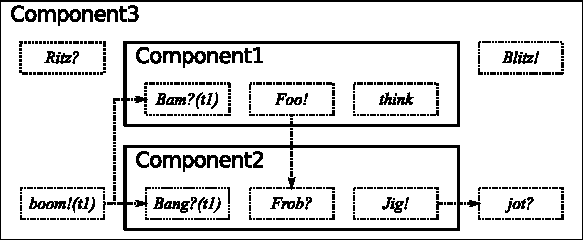
\includegraphics[width=\textwidth]{system_model}
\caption{Example remote sensor node expressed as a constellation of components, event handlers, and bindings.
  Components are depicted as solid rectangles, e.g., Remote Sensor.
  Event handlers are depicted as dotted rectangles, e.g., \emph{trigger!}.
  Output handlers are suffixed with \emph{!}, e.g., \emph{trigger!}.
  Input handlers are suffixed with \emph{?}, e.g., \emph{Trigger?}.
  Internal handlers have no suffix, e.g., \emph{compute}.
  Public handlers start with an uppercase letter, e.g., \emph{Trigger?}.
  Private events start with a lowercase letter, e.g., \emph{trigger!}.
  Bindings are indicate by dotted lines with an arrow pointing to the input.}
\label{sys_model}
\end{figure}

\paragraph{Example.}
Figure~\ref{sys_model} depicts a remote sensor node expressed as a constellation of components, event handlers, and bindings.
The Remote Sensor component consists of a Control component and three Channel components representing three network connections.
The Control component consists of a Sensor component, a Filter component, and a Statistics component.
The Control component starts the sampling process with the private uv-up output $Control.trigger!$.
The public uv-up input $Sensor.Trigger?$ is executed atomically with $Control.trigger!$ due to the binding $Control.trigger! \to (Sensor.Trigger?)$.
When the sampling process is complete, the public v-up output $Sensor.Sample!(f)$ distributes the sample $f$ to the Filter and Statistics components via the $Sensor.Sample!(f) \to (Filter.In?(t), Statistics.In?(u))$ binding.
Note that $f$, $t$, and $u$ must be of the same type.
The Filter component passes the filtered sample to the Control component via the $Filter.Out!(f) \to Control.sample?(f)$ binding which is owned by the Control component since $Control.sample?(f)$ is private.
The Statistics component calculates the statistics incrementally using the up internal $Statistics.compute$.
The statistics can be polled by the Control component using the $Control.request! \to (Statistics.Request?)$ and $Statistics.Response!(s) \to (Control.response?(s))$ bindings.
The Control component contains a public vp-output $Control.Send![](m)$ and a public vp-input $Control.Recv?[](m)$ for sending and receiving network messages using Channel components.
The parameters, i.e., 0, 1, and 2, are used to route messages to the appropriate network using the session idea outlined previously.
Opportunities for concurrent execution exist for the remote sensor depicted in figure~\ref{sys_model}.
The set of components implied by $Control.trigger!$ is $(Control, Sensor)$ while the set of components implied by $Statistics.compute$ is $(Statistics)$.
Since the sets are disjoint, the two actions can be executed concurrently.

\subsection{Formalization as I/O Automata}

The Input/Output (I/O) automata model was developed by Lynch~\cite{lynch1996distributed} to model reactive concurrent and asynchronous systems.
An I/O automaton consists of state variables and atomic actions that manipulate the state.
The three action types are inputs, outputs, and internal actions.
Input actions receive a signal or a value and output actions produce a signal or a value.
Internal actions just manipulate the state of the automaton.
Output and internal actions are \emph{locally controlled actions}~\cite{lynch1996distributed} are often presented as precondition and an effect.
The precondition is a predicate over the state variables that enables the effect when selected.
The effect is a function that computes the next state of the automaton from the current state.
Input and output actions are \emph{external actions}~\cite{lynch1996distributed} because they allow an automaton to communicate with other automata.
Automata may \emph{composed} by concatenating the state variables of the constituent automata and incorporating the effects of input actions into output actions with the same name.
A useful operation in composite automata is \emph{hiding}~\cite{lynch1996distributed} which converts an output action to an internal action.
Composing automata results in a static configuration, i.e., the set of automata and their interactions are fixed.
Execution in the I/O automata model consists of repeatedly selecting a local action and then applying the effect if the precondition is true.
The scheduler is assumed to be fair meaning that a local action is guaranteed to be selected (but not executed) infinitely often.

The proposed system has a straightforward mapping to the I/O automata model: components are automata and event handlers are actions.
